\chapter{需求分析}
本项目的需求分析方面很简单,也很明确。这里选用数据流图(DFD)来表达。
\begin{center}
  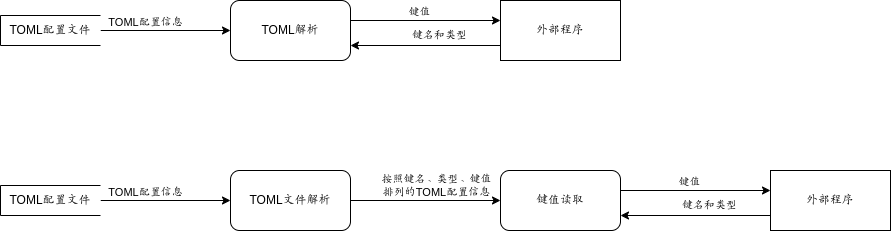
\includegraphics[width=\textwidth]{images/数据流图.png}
\end{center}

此图由draw.io绘图工具绘制后导出。


\chapter{设计}


\section{流程图}
本项目规模很小,并且使用的编程语言是面向结构的C语言,所以使用流程图来设计。

下面的流程图是针对本项目中的示例程序,在实际使用中,读取文件方面的操作由相关调用代码自行处理。
\begin{center}
  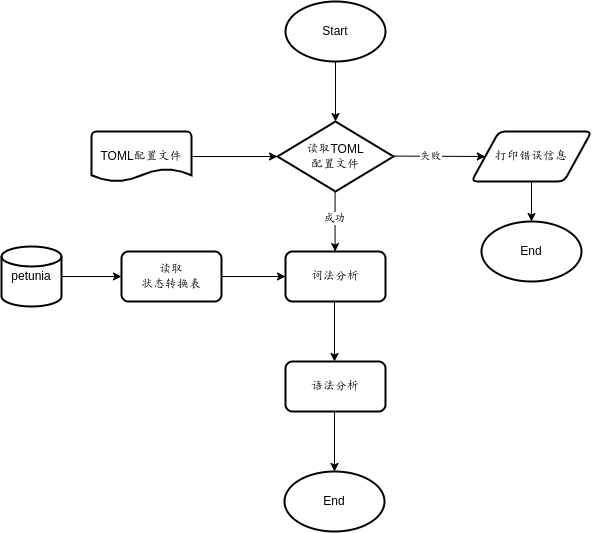
\includegraphics[width=0.8\textwidth]{images/流程图.png}
\end{center}


\section{词法分析}


\subsection{状态转换图}


\subsubsection{注释(comment)}
\noindent
\begin{tikzpicture}[node distance=9em, align=center]
  \node[state,initial]    (s001)               {$001$};
  \node[state]            (s101)[right=of s001]{$101$};
  \node[state, accepting] (s102)[right=of s101]{$102$};
  \path[->](s001) edge [loop above] node[text width=5em] {space, $\backslash$t, $\backslash$n, $\backslash$r} ()
                 edge node [above] {\#} (s101)
           (s101) edge [loop above] node[text width=12em] {characters containing tabs but no other control characters($\backslash$0x00$\sim\backslash$0x08, $\backslash$ 0x0A$\sim\backslash$0x1F, $\backslash$0x7F)} ()
                  edge node[above] {$\backslash$n} (s102);
\end{tikzpicture}


\subsubsection{祼键(bare key)}
\noindent
\begin{tikzpicture}[align=center]
  \node[state,initial]    (s001)               {$001$};
  \node[state]            (s201)[right=7em of s001]{$201$};
  \node[state, accepting] (s202)[right=12em of s201]{$202$};
  \path[->](s001) edge [loop above] node[text width=5em] {space, $\backslash$t, $\backslash$n, $\backslash$r} ()
                  edge node [above, text width=7em] {letter, \_, digit, -} (s201)
           (s201) edge [loop above] node[text width=5em] {letter, \_, digit, -}()
                  edge node[above, text width=12em] {character that are not letter, digit, underscore, and dash.} (s202);
\end{tikzpicture}


\subsubsection{运算符}
等号(=):

\noindent
\begin{tikzpicture}[align=center]
  \node[state,initial]    (s001)               {$001$};
  \node[state]            (s301)[right=of s001]{$301$};
  \node[state, accepting] (s302)[right=of s301]{$302$};
  \path[->](s001) edge [loop above] node[text width=5em] {space, $\backslash$t, $\backslash$n, $\backslash$r} ()
                  edge node [above] {=} (s301)
           (s301) edge node[above] {all} (s302);
\end{tikzpicture}


\subsubsection{字符串(string)}
\noindent
\begin{tikzpicture}[align=center]
  \node[state,initial]    (s001)               {$001$};
  \node[state]            (s401)[right=6em of s001]{$401$};
  \node[state]            (s402)[below=8ex of s401]{$402$};
  \node[state, accepting] (s403)[right=6em of s401]{$403$};
  \path[->](s001) edge [loop above] node[text width=5em] {space, $\backslash$t, $\backslash$n, $\backslash$r} ()
                  edge node [above] {"} (s401)
           (s401) edge [loop above] node[text width=10em] {character that are not ", $\backslash$, $\backslash$0x00$\sim\backslash$0x08, $\backslash$0x0A$\sim\backslash$0x1F, $\backslash$0x7F}()
                  edge [bend right] node[left] {$\backslash$}(s402)
                  edge node[above] {"} (s403)
           (s402) edge [bend right] node[right] {$\backslash$, "}(s401);
\end{tikzpicture}

按照当前的实际需要,暂时不支持多行字符串,另外转义字符目前也只支持反斜杠和双引号。


\subsubsection{整数(integer)}
\noindent
\begin{tikzpicture}[align=center]
  \node[state,initial]    (s001)               {$001$};
  \node[state]            (s501)[right=6em of s001]{$501$};
  \node[state]            (s502)[below=8ex of s501]{$502$};
  \node[state, accepting] (s503)[right=8em of s501]{$503$};
  \path[->](s001) edge [loop above] node[text width=5em] {space, $\backslash$t, $\backslash$n, $\backslash$r} ()
                  edge node [above] {digit, +, -} (s501)
           (s501) edge [loop above] node {digit}()
                  edge [bend right] node[left] {underline}(s502)
                  edge node[above, text width=8em] {non-numeric characters} (s503)
           (s502) edge [bend right] node[right] {digit}(s501);
\end{tikzpicture}

目前暂时不支持16进制、8进制。


\subsubsection{浮点数(fractional)}
\noindent
\begin{tikzpicture}[align=center]
  \node[state,initial]    (s001)               {$001$};
  \node[state]            (s501)[right=4em of s001]{$501$};
  \node[state]            (s502)[below=8ex of s501]{$502$};
  \node[state]            (s601)[right=5em of s501]{$601$};
  \node[state, accepting] (s602)[right=6em of s601]{$602$};
  \node[state]            (s603)[below=8ex of s601]{$603$};
  \node[state]            (s604)[right=6em of s603]{$604$};
  \node[state, accepting] (s605)[right=6em of s604]{$605$};
  \node[state]            (s606)[below right=4em of s603]{$606$};
  \path[->](s001) edge [loop above] node[text width=5em] {space, $\backslash$t, $\backslash$n, $\backslash$r} ()
                  edge node[above, text width=4em] {digit, +, -} (s501)
           (s501) edge [loop above] node {digit}()
                  edge [bend right] node[left] {underline}(s502)
                  edge node[above, text width=4em] {decimal point} (s601)
           (s502) edge [bend right] node[right] {digit}(s501)
           (s601) edge node[above, text width=6em] {characters other than digits, E, e} (s602)
                  edge node[right] {E, e} (s603)
           (s603) edge node[above] {digit} (s604)
                  edge node[right] {+, -} (s606)
           (s606) edge node[right] {digit} (s604)
           (s604) edge node[above, text width=6em] {characters other than digits, E, e} (s605);
\end{tikzpicture}


\subsubsection{界符}
左中括号:

\begin{tikzpicture}[align=center]
  \node[state,initial]    (s001)               {$001$};
  \node[state]            (s701)[right=of s001]{$701$};
  \node[state, accepting] (s702)[right=of s701]{$702$};
  \path[->](s001) edge [loop above] node[text width=5em] {space, $\backslash$t, $\backslash$n, $\backslash$r} ()
                  edge node [above] {[} (s701)
           (s701) edge node [above] {all} (s702);
\end{tikzpicture}

右中括号:

\begin{tikzpicture}[align=center]
  \node[state,initial]    (s001)               {$001$};
  \node[state]            (s703)[right=of s001]{$703$};
  \node[state, accepting] (s704)[right=of s703]{$704$};
  \path[->](s001) edge [loop above] node[text width=5em] {space, $\backslash$t, $\backslash$n, $\backslash$r} ()
                  edge node [above] {]} (s703)
           (s703) edge node [above] {all} (s704);
\end{tikzpicture}

逗号:

\begin{tikzpicture}[align=center]
	\node[state,initial]    (s001)               {$001$};
	\node[state]            (s705)[right=of s001]{$705$};
	\node[state, accepting] (s706)[right=of s703]{$706$};
	\path[->](s001) edge [loop above] node[text width=5em] {space, $\backslash$t, $\backslash$n, $\backslash$r} ()
	edge node [above] {,} (s705)
	(s703) edge node [above] {all} (s706);
\end{tikzpicture}


\subsection{用于TOML状态转换表解析的状态转换图}
这个标题有些绕,实际对应的是上一节的内容。上一节的状态转换图最后是要用一张状态转换表(这里使用CSV文件)来实现的,那么这张表在程序读入时,需要把表文件中的内容转换保存在C语言的数组中。但是,因为这张表文件的内容会包含不能被直接转换的内容,比如一些不可见的控制字符,所以就需要做一些加工转换。这样一来,在我们的程序中就又增加了一个词法分析,只是比较简单,并且在具体实现时将不再把这个转换规则以外部文件的形式存放,而是直接编写在程序中。

这里的状态转换,核心部分就是转义字符的处理。

\begin{tikzpicture}[align=center]
	\node[state,initial]    (s001)               {$001$};
	\node[state]            (s101)[right=of s001]{$101$};
	\node[state, accepting] (s102)[right=8em of s101]{$102$};
	\node[state, accepting] (s103)[below=4ex of s101]{$103$};
	\path[->](s001) edge node[above] {$\backslash$} (s101)
	                edge node[right] {other} (s103)
	         (s101) edge node[above] {t, n, r, ", $\backslash$} (s102);
\end{tikzpicture}